\documentclass[letterpaper,12pt,fleqn]{article}
\usepackage{matharticle}
\usepackage{graphtheory}
\pagestyle{empty}
\begin{document}
\section*{1.3: Common Classes of Graphs}

\begin{enumerate}[start=21]
\item Draw the graph \(3P_4\cup2C_4\cup K_4\).

  \begin{tikzpicture}[every node/.style={unlabeled node}]
    \pathN{4}{(0,-2.5)}{above}{};
    \pathN{4}{(1.5,-2.5)}{above}{};
    \pathN{4}{(3,-2.5)}{above}{};
    \cycleN{4}{(5,0)}{0.5in}{135}{};
    \cycleN{4}{(7.5,0)}{0.5in}{135}{};
    \completeN{4}{(10,0)}{0.5in}{135}{};
  \end{tikzpicture}

  \bigskip

\item Let \(G\) be a disconnected graph.  By Theorem 1.11, \(\comp{G}\) is connected.  Prove that if \(u\) and \(v\)
  are any two vertices of \(\comp{G}\), then \(d_{\comp{G}}(u,v)=1\) or \(d_{\comp{G}}(u,v)=2\).  Therefore, if \(G\)
  is a disconnected graph, then \(\diam(\comp{G})\le2\).

  \begin{proof}
    Assume \(u,v\in V(G)\).

    \begin{description}
    \item[Case 1:] \(uv\notin E(G)\)

      \(\therefore uv\in E(\comp{G})\) and thus \(d_{\comp{G}}(u,v)=1\).
      
    \item[Case 2:] \(uv\in E(G)\)

      This means that \(u\) and \(v\) are in the same component in \(G\).  Furthermore, \(uv\notin E(\comp{G})\).
      However, since \(G\) is disconnected, there exists a distinct vertex \(w\) in a different component in \(G\),
      and so \(uw,vw\in E(\comp{G})\).  Consider the path \((u,w,v)\).  This is a \(u-v\) path in \(\comp{G}\) of
      length \(2\).

      \(\therefore d_{\comp{G}}(u,v)=2\)
    \end{description}

    \(\therefore\diam(\comp{G})\le2\)
  \end{proof}

\item Consider the following question: For a given positive integer \(k\), does there exist a connected graph \(G\)
  whose complement \(\comp{G}\) is also connected and contains four distinct vertices \(u,v,x,y\) for which
  \(d_G(u,v)=k=d_{\comp{G}}(x,y)\)?
  \begin{enumerate}
  \item Show that the answer to this question is yes if \(k=1\) or \(k=2\).

    For \(k=1\):

    \begin{minipage}{2.5in}
      \begin{center}
        \begin{tikzpicture}[every node/.style={labeled node}]
          \cycleV{\(u\),\(v\),\(x\),\(w\),\(y\)}{(0,0)}{0.75in}{90}{}
        \end{tikzpicture}

        \(G\)
      \end{center}
    \end{minipage}
    \begin{minipage}{2.5in}
      \begin{center}
        \begin{tikzpicture}[every node/.style={labeled node}]
          \cycleVnodes{\(u\),\(v\),\(x\),\(w\),\(y\)}{(0,0)}{0.75in}{90}{}
          \draw (1) to (3) to (5) to (2) to (4) to (1);
        \end{tikzpicture}

        \(\comp{G}\)
      \end{center}
    \end{minipage}

    \bigskip

    For \(k=2\):

    \begin{minipage}{2.5in}
      \begin{center}
        \begin{tikzpicture}[every node/.style={labeled node}]
          \cycleV{\(u\),\(x\),\(y\),\(v\),\(w\)}{(0,0)}{0.75in}{90}{}
        \end{tikzpicture}

        \(G\)
      \end{center}
    \end{minipage}
    \begin{minipage}{2.5in}
      \begin{center}
        \begin{tikzpicture}[every node/.style={labeled node}]
          \cycleVnodes{\(u\),\(x\),\(y\),\(v\),\(w\)}{(0,0)}{0.75in}{90}{}
          \draw (1) to (3) to (5) to (2) to (4) to (1);
        \end{tikzpicture}

        \(\comp{G}\)
      \end{center}
    \end{minipage}

    \bigskip

  \item Find the largest value of \(k\) for with the answer to this question is yes.

    For \(k\ge3\), it must be the case that \(uv\notin E(G)\).  Furthermore, it must be the case that \(xy\in
    E(G)\); otherwise, \(xy\in E(\comp{G})\) and \(d_{\comp{G}}(x,y)=1\).  If \(G\) contains any vertex \(w\) such
    that \(wx,wy\notin E(G)\) then there is always a \((x,w,y)\) path of length 2 in \(\comp{G}\).  Thus \(u\) and
    \(v\) must be adjacent to \(x\) and \(y\), but neither can be adjacent to both, which would mean that
    \(d_G(u,v)=2\).  So \(G\) must contain a 4-path as follows:

    \bigskip

    \begin{center}
      \begin{tikzpicture}[every node/.style={labeled node},node distance={1in}]
        \pathV{\(u\),\(x\),\(y\),\(v\)}{(0,0)}{right}{};
      \end{tikzpicture}
    \end{center}

    \bigskip

    In \(\comp{G}\), this path would become:

    \bigskip

    \begin{center}
      \begin{tikzpicture}[every node/.style={labeled node},node distance={1in}]
        \pathVnodes{\(u\),\(x\),\(y\),\(v\)}{(0,0)}{right}{};
        \draw (1) edge [bend left] (3);
        \draw (1) edge [bend left] (4);
        \draw (2) edge [bend right] (4);
      \end{tikzpicture}
    \end{center}
    
    \bigskip

    Thus, \(d_{\comp{G}}(x,y)\le3\).

    Therefore, the maximum such \(k=3\).

  \end{enumerate}

\item Determine whether the graphs \(G_1\) and \(G_2\) of Figure 1.34 are bipartite.  If a graph is bipartite, then
  redraw it indicating the partite sets; if not, then give an explanation as to why the graph is not bipartite.

  \(G_1\) is bipartite:

  \begin{center}
    \begin{tikzpicture}
      \colorlet{cu}{green!25!white}
      \colorlet{cw}{red!25!white}
      \cycleNnodes{6}{(0,0)}{1in}{90}{c};
      \begin{scope}[every node/.style={labeled node},node distance=1in]
        \node [fill=cw] (v) at (c1) {\(v\)};
        \node [fill=cu] (w) at (c2) {\(w\)};
        \node [fill=cw] (z) at (c3) {\(z\)};
        \node [fill=cu] (y) at (c4) {\(y\)};
        \node [fill=cw] (x) at (c5) {\(x\)};
        \node [fill=cu] (u) at (c6) {\(u\)};
        \node [fill=cu] (r) [above left=0.5in and 1in of x] {\(r\)};
        \node [fill=cu] (q) [below left=0.5in and 1in of x] {\(q\)};
        \node [fill=cw] (s) [right=of w] {\(s\)};
        \node [fill=cu] (t) [right=of z] {\(t\)};
      \end{scope}
      \draw (u) to (x) to (y) to (z) to (w) to (v) to (u);
      \draw (x) to (r);
      \draw (x) to (q);
      \draw (w) to (s) to (t) to (z);
      \draw (u) to (z);
      \draw (x) to (w);
    \end{tikzpicture}

    \bigskip

    \(G_1\)
  \end{center}

  \bigskip

  \(G_2\) is not bipartite since it contains an odd cycle: \((u,v,w,r,x,u)\).

  \bigskip

  \begin{center}
    \begin{tikzpicture}
      \cycleNnodes{6}{(0,0)}{1in}{90}{c};
      \begin{scope}[every node/.style={labeled node},node distance=1in]
        \node (r) at (0,0) {\(r\)};
        \node (v) at (c1) {\(v\)};
        \node (w) at (c2) {\(w\)};
        \node (z) at (c3) {\(z\)};
        \node (y) at (c4) {\(y\)};
        \node (x) at (c5) {\(x\)};
        \node (u) at (c6) {\(u\)};
        \node (s) [right=of w] {\(s\)};
        \node (t) [right=of z] {\(t\)};
      \end{scope}
      \draw (w) to (z) to (y) to (x);
      \draw (w) to (s) to (t) to (z);
      \draw [red] (u) to (v) to (v) to (w) to (r) to (x) to (u);
    \end{tikzpicture}

    \bigskip

    \(G_1\)
  \end{center}

\item Let \(G\) be a graph of order 5 or more.  Prove that at most one of \(G\) and \(\comp{G}\) is bipartite.

  \begin{proof}
    AWLOG: \(G\) is bipartite.

    Since \(n=5\), there must be at least 3 vertices in at least one of the partite sets.  Since these vertices are
    not adjacent in \(G\), they will all be adjacent in \(\comp{G}\), thus forming a 3-cycle.

    \(\therefore\comp{G}\) is not bipartite.
  \end{proof}
  
\item Suppose that the vertex set of a graph \(G\) is a (finite) set of integers.  Two vertices \(x\) and \(y\) are
  adjacent if \(x+y\) is odd.  To which well-known class of graphs is \(G\) a member?

  Such a graph would be a bipartite graph, partitioning the vertices into even and odd partite sets.  This is
  because: E+E=E (not adjacent), O+O=E (not adjacent), and O+E=E+O=O (adjacent).

\item For the following pairs \(G,H\) of graphs, draw \(G+H\) and \(G\times H\).
  \begin{enumerate}
  \item \(G=K_5\) and \(H=K_2\)

    \bigskip

    \begin{minipage}{1.5in}
      \begin{center}
        \begin{tikzpicture}[every node/.style={unlabeled node}]
          \completeN{7}{(0,0)}{0.5in}{90}{};
        \end{tikzpicture}

        \bigskip

        \(K_5+K_2=K_7\)
      \end{center}
    \end{minipage}
    \begin{minipage}{4in}
      \begin{center}
        \begin{tikzpicture}[every node/.style={unlabeled node}]
          \completeN{5}{(0,0)}{0.5in}{90}{l};
          \completeN{5}{(1.5in,0)}{0.5in}{90}{r};
          \draw (l1) to (r1);
          \draw (l2) to (r5);
          \draw (l3) to (r4);
          \draw (l4) to ($(l4)-(0,0.25in)$) -| (r3);
          \draw (l5) to ($(l5)+(0,0.5in)$) -| (r2);
        \end{tikzpicture}

        \bigskip

        \(K_5\times K_2\)
      \end{center}
    \end{minipage}

    \bigskip

  \item \(G=\comp{K_5}\) and \(H=\comp{K_3}\)

    \bigskip

    \begin{minipage}{2.5in}
      \begin{center}
        \begin{tikzpicture}[every node/.style={unlabeled node}]
          \pathNnodes{5}{(0,-2)}{above}{l};
          \pathNnodes{3}{(2,-1)}{above}{r};
          \foreach \i in {1,2,3,4,5}{
            \foreach \j in {1,2,3}{
              \draw (l\i) edge (r\j);
            }
          }
        \end{tikzpicture}

        \bigskip

        \(\comp{K_5}+\comp{K_3}=K_{5,3}\)
      \end{center}
    \end{minipage}
    \begin{minipage}{2.5in}
      \begin{center}
        \begin{tikzpicture}[every node/.style={unlabeled node}]
          \pathNnodes{3}{(0,0)}{right}{};
          \pathNnodes{3}{(0,1)}{right}{};
          \pathNnodes{3}{(0,2)}{right}{};
          \pathNnodes{3}{(0,3)}{right}{};
          \pathNnodes{3}{(0,4)}{right}{};
        \end{tikzpicture}

        \bigskip

        \(\comp{K_5}\times\comp{K_3}=E_{15}\)
      \end{center}
    \end{minipage}

    \bigskip

  \item \(G=C_5\) and \(H=K_1\)

    \bigskip

    \begin{minipage}{2.5in}
      \begin{center}
        \begin{tikzpicture}[every node/.style={unlabeled node}]
          \cycleN{5}{(0,0)}{0.5in}{90}{};
          \node (c) at (0,0) {};
          \foreach \i in {1,2,3,4,5}{
            \draw (c) edge (\i);
          }
        \end{tikzpicture}

        \bigskip

        \(C_5+K_1\)
      \end{center}
    \end{minipage}
    \begin{minipage}{2.5in}
      \begin{center}
        \begin{tikzpicture}[every node/.style={unlabeled node}]
          \cycleN{5}{(0,0)}{0.5in}{90}{};
        \end{tikzpicture}

        \bigskip

        \(C_5\times K_1=C_5\)
      \end{center}
    \end{minipage}
  \end{enumerate}

  \bigskip

\item We have seen that for \(n\ge1\), the \(n\)-cube \(Q_n\) is that graph whose vertex set is the set of
  \(n\)-bit strings, where two vertices of \(Q_n\) are adjacent if they differ in exactly one coordinate.
  \begin{enumerate}
  \item For \(n\ge2\), define the graph \(R_n\) to be that graph whose vertex set is the set of \(n\)-bit strings,
    where two vertices of \(R_n\) are adjacent if they differ in exactly two coordinates.  Draw \(R_2\) and
    \(R_3\).

    \bigskip

    \begin{minipage}{2.5in}
      \begin{center}
        \begin{tikzpicture}[every node/.style={labeled node}]
          \cycleVnodes{\(00\),\(01\),\(10\),\(11\)}{(0,0)}{0.5in}{90}{};
          \draw (1) edge (4);
          \draw (2) edge (3);
        \end{tikzpicture}

        \bigskip

        \(R_2\)
      \end{center}
    \end{minipage}
    \begin{minipage}{3in}
      \begin{center}
        \begin{tikzpicture}[every node/.style={labeled node}]
          \cycleVnodes{\(000\),\(001\),\(010\),\(011\),\(100\),\(101\),\(110\),\(111\)}{(0,0)}{1.25in}{90}{};
          \draw (1) edge (4) edge (6) edge (7);
          \draw (2) edge (3) edge (5) edge (8);
          \draw (3) edge (8) edge (5);
          \draw (4) edge (7) edge (6);
          \draw (5) edge (8);
          \draw (6) edge (7);
        \end{tikzpicture}

        \bigskip

        \(R_3\)
      \end{center}
    \end{minipage}

    \bigskip
    
  \item For \(n\ge3\), define the graph \(S_n\) to be that graph whose vertex set is the set of \(n\)-bit strings,
    where two vertices of \(S_n\) are adjacent if they differ in exactly three coordinates.  Draw \(S_3\) and
    \(S_4\).

    \bigskip

    \begin{center}
      \begin{tikzpicture}[every node/.style={labeled node}]
        \cycleVnodes{\(000\),\(001\),\(010\),\(011\),\(100\),\(101\),\(110\),\(111\)}{(0,0)}{1in}{90}{};
        \draw (1) edge (8);
        \draw (2) edge (7);
        \draw (3) edge (6);
        \draw (4) edge (5);
      \end{tikzpicture}

      \bigskip

      \(S_3\)
    \end{center}

    \begin{center}
      \begin{tikzpicture}[every node/.style={labeled node}]
        \cycleVnodes{\(0000\),\(0001\),\(0010\),\(0011\),\(0100\),\(0101\),\(0110\),\(0111\),
          \(1000\),\(1001\),\(1010\),\(1011\),\(1100\),\(1101\),\(1110\),\(1111\)}{(0,0)}{2.5in}{90}{};
        \draw (1) edge (8) edge (12) edge (14) edge [bend right=1in] (15);
        \draw (2) edge (7) edge (11) edge (13) edge [bend right=1in] (16);
        \draw (3) edge (6) edge (10) edge (16) edge (13);
        \draw (4) edge (5) edge (9) edge (15) edge (14);
        \draw (5) edge (16) edge (10) edge (11);
        \draw (6) edge (15) edge (9) edge (12);
        \draw (7) edge (14) edge (12) edge [bend left=1in] (9);
        \draw (8) edge (13) edge (11) edge [bend left=1in] (10);
        \draw (9) edge (16);
        \draw (10) edge (15);
        \draw (11) edge (14);
        \draw (12) edge (13);
      \end{tikzpicture}

      \bigskip

      \(S_4\)
    \end{center}
  \end{enumerate}
  
\end{enumerate}

\end{document}
